\section{Formulation} \label{sec:formul}
The phase-field model as a diffuse interface model does not introduce discontinuities into the solid but the fracture surface is approximated by a scalar valued field. Thus, the boundary between damaged and not damaged areas is smoothed. In the following parts, a model for brittle and ductile fracture as well as a second- and fourth-order model are presented. At first, the notation and formulation considering brittle fracture is outlined. Afterwards, differences in the formulation considering ductile fracture are shown. For the rest of this paper, following notation is made (see ). The arbitraray body $\Omega\subset\mathbb{R}^{d}$ ($d\in\{1,2,3\}$) has external boundary $\partial\Omega$ and internal discontinuity boundary $\Gamma$. The displacement field at a given point $\mathbf{x}$ and time $t$ is given by $\mathbf{u}\left(\mathbf{x},t\right)\in\mathbb{R}^{d}$. Dirichlet boundary conditions $\mathbf{u}\left(\mathbf{x},t\right)=\mathbf{g}\left(\mathbf{x},t\right)$ on $\partial\Omega_{\mathbf{g}}$ and Neumann boundary conditions $\mathbf{t}\left(\mathbf{x},t\right)=\mathbf{h}\left(\mathbf{x},t\right)$ on $\partial\Omega_{\mathbf{h}}$ are imposed with $\partial\Omega_{\mathbf{g}}\cup\partial\Omega_{\mathbf{h}}=\partial\Omega$. $\mathbf{t}\left(\mathbf{x},t\right)$ describes a given traction vector force.

\begin{figure}[h]
    \centering
    \begin{subfigure}[t]{0.5\textwidth}
        \centering
        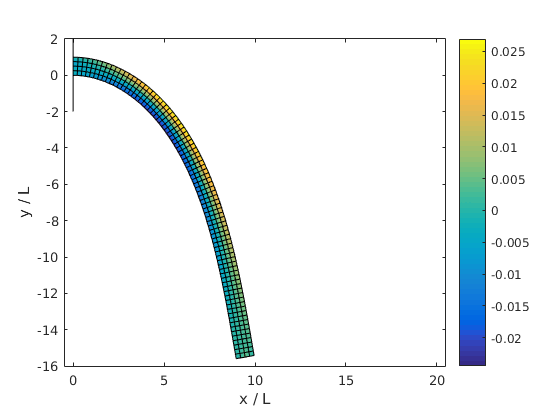
\includegraphics[width=5cm]{data/a}
        \caption{}\label{a}
    \end{subfigure}%
    ~ 
    \begin{subfigure}[t]{0.5\textwidth}
        \centering
        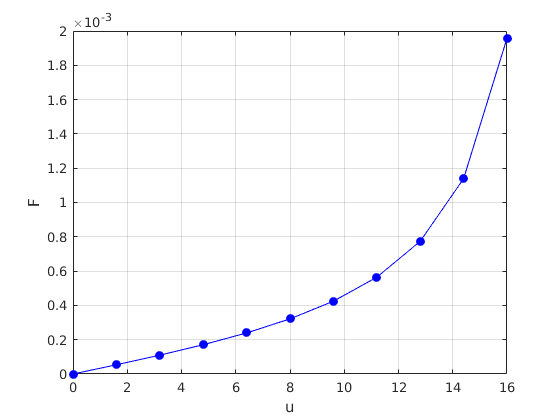
\includegraphics[width=5cm]{data/b}
        \caption{}\label{b}
    \end{subfigure}
    \caption{Caption place holder \subrefnew{a} \subrefnew{b}} \label{fig}
\end{figure}
\\
\figref{fig}\subrefnew{a}

\subsection{Griffith's theory of brittle fracture} \label{sec:formul_Griffith}
Considering small derformations and deformation gradients, the small strain tensor $\mathbf{\epsilon}\left(\mathbf{x},t\right)$ is given by
\begin{equation}
	\bm{\varepsilon} = \nabla^{s}\mathbf{u}
\end{equation}
where $\cdot^{s}$ refers to the symmetric part. Considering isotropic linear elasticity, the undamaged elastic energy densitiy can be expressed by
\begin{equation}
	\Psi_ {e}\left(\bm{\varepsilon}\right) = \dfrac{1}{2}\lambda tr\left(\bm{\varepsilon}\right)^{2}+\mu\bm{\varepsilon}:\bm{\varepsilon}
\end{equation}
using the Lam\'{e} constants $\lambda$ and $\mu$.